% Created by tikzDevice version 0.10.1 on 2018-06-27 15:02:47
% !TEX encoding = UTF-8 Unicode
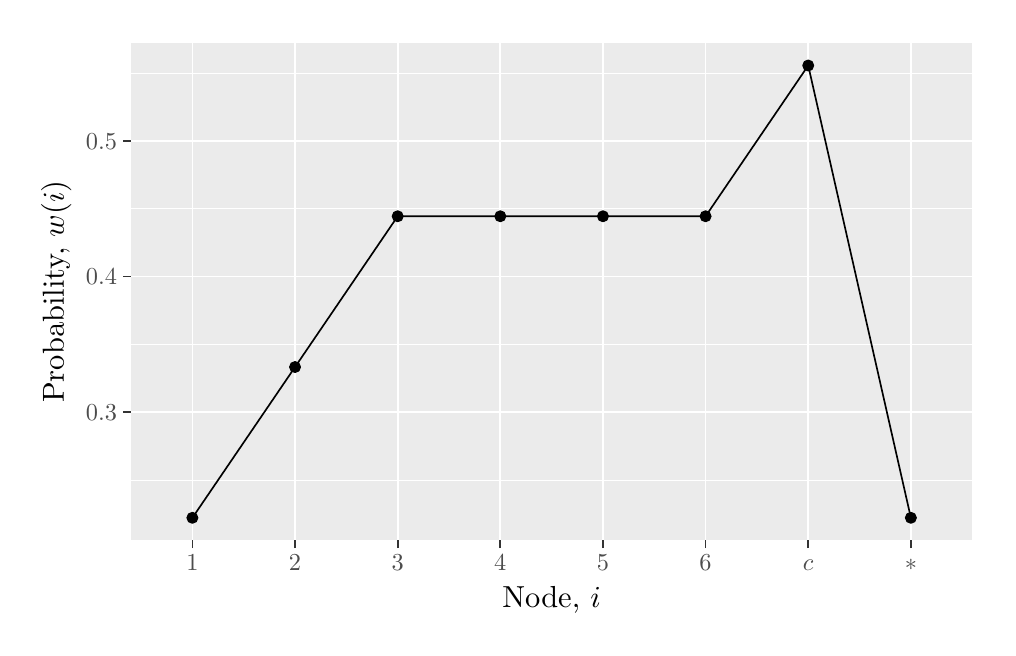
\begin{tikzpicture}[x=1pt,y=1pt]
\definecolor{fillColor}{RGB}{255,255,255}
\path[use as bounding box,fill=fillColor,fill opacity=0.00] (0,0) rectangle (346.90,216.81);
\begin{scope}
\path[clip] (  0.00,  0.00) rectangle (346.90,216.81);
\definecolor{drawColor}{RGB}{255,255,255}
\definecolor{fillColor}{RGB}{255,255,255}

\path[draw=drawColor,line width= 0.6pt,line join=round,line cap=round,fill=fillColor] (  0.00,  0.00) rectangle (346.90,216.81);
\end{scope}
\begin{scope}
\path[clip] ( 37.27, 31.53) rectangle (341.40,211.31);
\definecolor{fillColor}{gray}{0.92}

\path[fill=fillColor] ( 37.27, 31.53) rectangle (341.40,211.31);
\definecolor{drawColor}{RGB}{255,255,255}

\path[draw=drawColor,line width= 0.3pt,line join=round] ( 37.27, 53.32) --
	(341.40, 53.32);

\path[draw=drawColor,line width= 0.3pt,line join=round] ( 37.27,102.35) --
	(341.40,102.35);

\path[draw=drawColor,line width= 0.3pt,line join=round] ( 37.27,151.38) --
	(341.40,151.38);

\path[draw=drawColor,line width= 0.3pt,line join=round] ( 37.27,200.41) --
	(341.40,200.41);

\path[draw=drawColor,line width= 0.6pt,line join=round] ( 37.27, 77.84) --
	(341.40, 77.84);

\path[draw=drawColor,line width= 0.6pt,line join=round] ( 37.27,126.87) --
	(341.40,126.87);

\path[draw=drawColor,line width= 0.6pt,line join=round] ( 37.27,175.90) --
	(341.40,175.90);

\path[draw=drawColor,line width= 0.6pt,line join=round] ( 59.52, 31.53) --
	( 59.52,211.31);

\path[draw=drawColor,line width= 0.6pt,line join=round] ( 96.61, 31.53) --
	( 96.61,211.31);

\path[draw=drawColor,line width= 0.6pt,line join=round] (133.70, 31.53) --
	(133.70,211.31);

\path[draw=drawColor,line width= 0.6pt,line join=round] (170.79, 31.53) --
	(170.79,211.31);

\path[draw=drawColor,line width= 0.6pt,line join=round] (207.88, 31.53) --
	(207.88,211.31);

\path[draw=drawColor,line width= 0.6pt,line join=round] (244.96, 31.53) --
	(244.96,211.31);

\path[draw=drawColor,line width= 0.6pt,line join=round] (282.05, 31.53) --
	(282.05,211.31);

\path[draw=drawColor,line width= 0.6pt,line join=round] (319.14, 31.53) --
	(319.14,211.31);
\definecolor{drawColor}{RGB}{0,0,0}
\definecolor{fillColor}{RGB}{0,0,0}

\path[draw=drawColor,line width= 0.4pt,line join=round,line cap=round,fill=fillColor] ( 59.52, 39.70) circle (  1.96);

\path[draw=drawColor,line width= 0.4pt,line join=round,line cap=round,fill=fillColor] ( 96.61, 94.18) circle (  1.96);

\path[draw=drawColor,line width= 0.4pt,line join=round,line cap=round,fill=fillColor] (133.70,148.66) circle (  1.96);

\path[draw=drawColor,line width= 0.4pt,line join=round,line cap=round,fill=fillColor] (170.79,148.66) circle (  1.96);

\path[draw=drawColor,line width= 0.4pt,line join=round,line cap=round,fill=fillColor] (207.88,148.66) circle (  1.96);

\path[draw=drawColor,line width= 0.4pt,line join=round,line cap=round,fill=fillColor] (244.96,148.66) circle (  1.96);

\path[draw=drawColor,line width= 0.4pt,line join=round,line cap=round,fill=fillColor] (282.05,203.14) circle (  1.96);

\path[draw=drawColor,line width= 0.4pt,line join=round,line cap=round,fill=fillColor] (319.14, 39.70) circle (  1.96);

\path[draw=drawColor,line width= 0.6pt,line join=round] ( 59.52, 39.70) --
	( 96.61, 94.18) --
	(133.70,148.66) --
	(170.79,148.66) --
	(207.88,148.66) --
	(244.96,148.66) --
	(282.05,203.14) --
	(319.14, 39.70);
\end{scope}
\begin{scope}
\path[clip] (  0.00,  0.00) rectangle (346.90,216.81);
\definecolor{drawColor}{gray}{0.30}

\node[text=drawColor,anchor=base east,inner sep=0pt, outer sep=0pt, scale=  0.88] at ( 32.32, 74.81) {0.3};

\node[text=drawColor,anchor=base east,inner sep=0pt, outer sep=0pt, scale=  0.88] at ( 32.32,123.84) {0.4};

\node[text=drawColor,anchor=base east,inner sep=0pt, outer sep=0pt, scale=  0.88] at ( 32.32,172.87) {0.5};
\end{scope}
\begin{scope}
\path[clip] (  0.00,  0.00) rectangle (346.90,216.81);
\definecolor{drawColor}{gray}{0.20}

\path[draw=drawColor,line width= 0.6pt,line join=round] ( 34.52, 77.84) --
	( 37.27, 77.84);

\path[draw=drawColor,line width= 0.6pt,line join=round] ( 34.52,126.87) --
	( 37.27,126.87);

\path[draw=drawColor,line width= 0.6pt,line join=round] ( 34.52,175.90) --
	( 37.27,175.90);
\end{scope}
\begin{scope}
\path[clip] (  0.00,  0.00) rectangle (346.90,216.81);
\definecolor{drawColor}{gray}{0.20}

\path[draw=drawColor,line width= 0.6pt,line join=round] ( 59.52, 28.78) --
	( 59.52, 31.53);

\path[draw=drawColor,line width= 0.6pt,line join=round] ( 96.61, 28.78) --
	( 96.61, 31.53);

\path[draw=drawColor,line width= 0.6pt,line join=round] (133.70, 28.78) --
	(133.70, 31.53);

\path[draw=drawColor,line width= 0.6pt,line join=round] (170.79, 28.78) --
	(170.79, 31.53);

\path[draw=drawColor,line width= 0.6pt,line join=round] (207.88, 28.78) --
	(207.88, 31.53);

\path[draw=drawColor,line width= 0.6pt,line join=round] (244.96, 28.78) --
	(244.96, 31.53);

\path[draw=drawColor,line width= 0.6pt,line join=round] (282.05, 28.78) --
	(282.05, 31.53);

\path[draw=drawColor,line width= 0.6pt,line join=round] (319.14, 28.78) --
	(319.14, 31.53);
\end{scope}
\begin{scope}
\path[clip] (  0.00,  0.00) rectangle (346.90,216.81);
\definecolor{drawColor}{gray}{0.30}

\node[text=drawColor,anchor=base,inner sep=0pt, outer sep=0pt, scale=  0.88] at ( 59.52, 20.52) {$1$};

\node[text=drawColor,anchor=base,inner sep=0pt, outer sep=0pt, scale=  0.88] at ( 96.61, 20.52) {$2$};

\node[text=drawColor,anchor=base,inner sep=0pt, outer sep=0pt, scale=  0.88] at (133.70, 20.52) {$3$};

\node[text=drawColor,anchor=base,inner sep=0pt, outer sep=0pt, scale=  0.88] at (170.79, 20.52) {$4$};

\node[text=drawColor,anchor=base,inner sep=0pt, outer sep=0pt, scale=  0.88] at (207.88, 20.52) {$5$};

\node[text=drawColor,anchor=base,inner sep=0pt, outer sep=0pt, scale=  0.88] at (244.96, 20.52) {$6$};

\node[text=drawColor,anchor=base,inner sep=0pt, outer sep=0pt, scale=  0.88] at (282.05, 20.52) {$c$};

\node[text=drawColor,anchor=base,inner sep=0pt, outer sep=0pt, scale=  0.88] at (319.14, 20.52) {$*$};
\end{scope}
\begin{scope}
\path[clip] (  0.00,  0.00) rectangle (346.90,216.81);
\definecolor{drawColor}{RGB}{0,0,0}

\node[text=drawColor,anchor=base,inner sep=0pt, outer sep=0pt, scale=  1.10] at (189.33,  7.44) {Node, $i$};
\end{scope}
\begin{scope}
\path[clip] (  0.00,  0.00) rectangle (346.90,216.81);
\definecolor{drawColor}{RGB}{0,0,0}

\node[text=drawColor,rotate= 90.00,anchor=base,inner sep=0pt, outer sep=0pt, scale=  1.10] at ( 13.08,121.42) {Probability, $w(i)$};
\end{scope}
\end{tikzpicture}
